% ===========================================================================
% TASTI 2026 extended abstract
%
%   Track  : 0201 Earth Observation and Remote Sensing (see docs/abstract_notes.md)
%   Budget : body 300-800 words, title <= 50 words, keywords <= 5
%   Build  : `make`            -> abstract.pdf (converts figures first)
%            `make wordcount`  -> body word count, floats and comments excluded
%
% Before editing the numbers, read docs/results.md (the S1/S2/S3 series must
% never be mixed). Before editing the wording, read docs/abstract_notes.md
% ("表現上の注意" has 9 rules that this text already satisfies).
%
% Line breaks inside a paragraph are insignificant to LaTeX, so this file uses
% semantic line breaks: one sentence per line, long sentences folded at clause
% boundaries. Paragraphs are separated by a blank line.
% ===========================================================================
\documentclass[a4paper]{article}
\usepackage{tasti2026}

\begin{document}

% ---------------------------------------------------------------------------
% Title block
% ---------------------------------------------------------------------------
\abstracttitle{%
  Accelerating Open-Source InSAR Time-Series Analysis on Consumer GPUs:
  A PyTorch-Based Network Inversion Solver for MintPy}

\abstractauthors{Syota Sasaki\affmark{*,1}}
\abstractaffil{\affmark{1}Earthsea Wizard, Japan}
\abstractemail{syota.sasaki@earthsea-wizard.com}
\abstractkeywords{InSAR, GPU acceleration, PyTorch, time-series analysis, open-source software}

% BODY-START

% ---------------------------------------------------------------------------
% Paragraph 1 -- Objective
%   The bottleneck (43.5% of a full run) and the accessibility constraint.
% ---------------------------------------------------------------------------
Interferometric SAR (InSAR) time-series analysis has become a standard tool
for measuring ground deformation from volcanoes, earthquakes, and land subsidence.
With the continuous acquisitions of Sentinel-1
and the arrival of the NASA-ISRO SAR Mission (NISAR) [1],
interferometric data are accumulating faster
than the throughput of the software that consumes them.
MintPy [2], one of the most widely used open-source packages
for small-baseline (SBAS) time-series analysis,
spends 43.5\% of a complete SBAS processing run in a single step:
the least-squares inversion of the interferogram network into a displacement
time series, solved pixel by pixel on the CPU.
The objective of this work is to remove that bottleneck with GPU acceleration
while keeping the software accessible---no HPC cluster,
no CUDA programming on the user side,
and no change to the default CPU behavior.

% ---------------------------------------------------------------------------
% Paragraph 2 -- Methodology
%   1.43x = CPU-relative, GPU port of the QR solver.
%   EVERY ratio in this abstract is CPU-relative by design. The S1 series
%   (same-GPU QR -> Cholesky: 16.5x internal, 4.49x step) was deliberately
%   removed so a first-time reader never has to switch baselines: the
%   1.43x -> 36.4x contrast carries "the shape, not the hardware" on its own.
%   Do NOT reintroduce it here. See docs/abstract_notes.md, note 2.
% ---------------------------------------------------------------------------
A direct port of the existing per-pixel least-squares routine
to a batched QR solver on the GPU reached only 1.43$\times$ over the CPU path:
the bottleneck was the shape of the problem, not the hardware.
Each pixel poses a $K \times P$ tall-skinny system,
and QR sweeps it one column at a time,
so batching still leaves $P$ sequential steps per matrix.
The solver was therefore reformulated around the normal equations.
Forming the Gram matrix and factorizing it is an established strategy
for parallel and GPU environments,
where it reduces the work to level-3 BLAS operations
and minimizes communication, at the documented cost of squaring
the condition number [3, 4];
here only the normal-equation solution, not a QR factor, is computed.
A single matrix multiplication reduces each $K \times P$ system
to a small $P \times P$ Gram block,
and full-rank blocks are factorized in one batched Cholesky call
in single precision using PyTorch [5],
with chunks sized to the available GPU memory (Fig.~1).
The implementation is deliberately minimally invasive:
it lives in a separate GPU subpackage,
is selected by a single configuration key,
and leaves the CPU path byte-for-byte unchanged.
The same core was reused for the DEM-error correction step
by substituting the design matrix.

% ---------------------------------------------------------------------------
% Figure 1 -- the mechanism (caption carries the three S1 qualifiers)
% ---------------------------------------------------------------------------
\begin{figure}[ht]
  \centering
  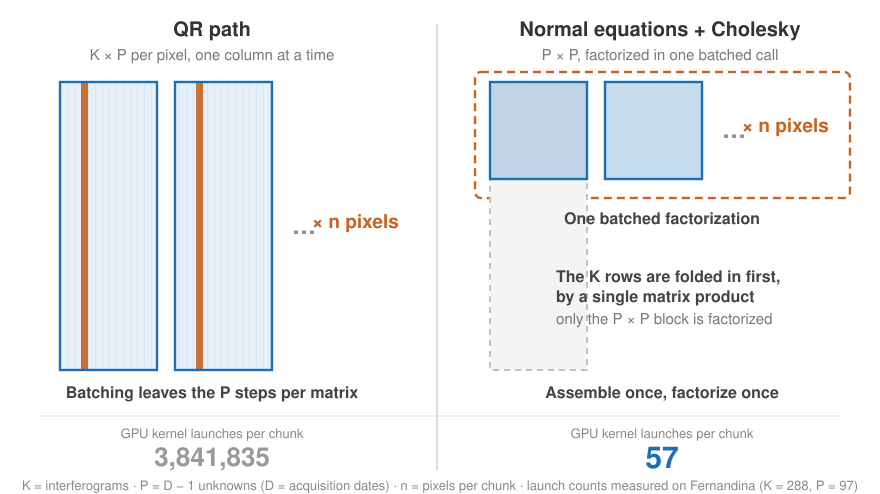
\includegraphics[width=0.92\textwidth]{figures/fig1_batched_cholesky.pdf}
  \caption{%
    Why the normal-equation path batches and the QR path does not.
    Launch counts are measured on the Fernandina scene ($K = 288$, $P = 97$).}
\end{figure}

% ---------------------------------------------------------------------------
% Paragraph 3a -- Key results, speed (run-in heading)
%   All numbers here are CPU-relative: S2 (Galapagos) and S3 (Table 1).
%   Do NOT claim a size dependence -- it does not hold; see docs/results.md.
% ---------------------------------------------------------------------------
\Needspace{4\baselineskip}
\textbf{Speedup.}
Every speedup reported here is measured against the CPU reference path,
on a consumer workstation GPU (NVIDIA GeForce RTX 5080, 16~GB).
In a controlled single-scene benchmark on a large Gal\'apagos scene
(3.4 million pixels, 475 retained interferograms), the inversion step fell
from 6{,}189~s to 170~s---a 36.4$\times$ step-level
and 44.4$\times$ kernel-level speedup---within 7.6~GB of GPU memory.
Separately, Table~1 reports step-level timings extracted from complete runs
on five public scenes spanning four interferometric processors,
two radar wavelengths, and more than an order of magnitude in scene size;
every scene accelerated, with speedups of 5.3$\times$ to 93.8$\times$.
Applying the same core to the DEM-error correction gives 6.2$\times$
on the large scene, and the complete 18-step processing workflow
runs end-to-end with the GPU solver enabled.

% ---------------------------------------------------------------------------
% Table 1 -- the S3 series. Caption goes ABOVE the table (template rule).
% Source of record: docs/results.md, section S3.
% ---------------------------------------------------------------------------
\begin{table}[ht]
  \centering
  \caption{%
    Step-level wall time of the network inversion,
    extracted from complete end-to-end processing runs on five public scenes.
    $K$ = interferograms, $D$ = acquisition dates.
    Every scene clears the numerical agreement gate against the CPU reference,
    and all five are openly available on Zenodo
    (records 3952953, 4743058, 15814132, 3952917, 4265413, in order).}
  \small
  \begin{tabular}{llrrrrrr}
    \toprule
    Scene             & Processor / band & Pixels  & $K$  & $D$ & CPU (s) & GPU (s) & Speedup      \\
    \midrule
    Fernandina        & ISCE-2 / C       & 0.27\,M & 288  & 98  & 645.1   & 6.9     & 93.8$\times$ \\
    Gal\'apagos       & ISCE-2 / C       & 3.40\,M & 490  & 98  & 2976.7  & 79.4    & 37.5$\times$ \\
    San Francisco Bay & GMTSAR / C       & 0.33\,M & 1297 & 333 & 1080.4  & 17.4    & 62.0$\times$ \\
    Kuju              & ROI\_PAC / L     & 0.23\,M & 167  & 24  & 31.0    & 4.5     & 6.9$\times$  \\
    San Francisco     & ARIA / C         & 1.04\,M & 505  & 114 & 58.9    & 11.1    & 5.3$\times$  \\
    \bottomrule
  \end{tabular}
\end{table}

% ---------------------------------------------------------------------------
% Paragraph 3b -- Key results, correctness (run-in heading)
% ---------------------------------------------------------------------------
\textbf{Numerical validation.}
Agreement with the CPU reference is enforced by a gate
on the normalized root-mean-square difference of the resulting time series.
All five scenes clear the gate on the final quality-masked products,
with normalized RMS differences on the order of $10^{-5}$,
consistent with accumulated single-precision rounding.
On the controlled large-scene benchmark
the largest absolute RMS difference is about 16~$\mu$m,
nearly two orders of magnitude below the millimeter-scale displacements
the analysis is meant to recover,
and well below a representative atmospheric noise floor.

% ---------------------------------------------------------------------------
% Paragraph 4 -- Conclusion AND significance
%   The template requires "significance" explicitly, so this must not end as a
%   bare recap. FORMOSAT-9 stays here as regional context only: no resolution
%   figure, no claim about X-band time-series suitability (note 5).
% ---------------------------------------------------------------------------
Network inversions that took hours now finish in minutes
on hardware a single research group can own,
and the normal-equation formulation introduces only micrometer-scale
differences---far below what the measurement itself can resolve.
Shortening the path from acquisition to a usable deformation time series
matters most where compute resources are limited:
rapid-response monitoring of volcanoes and earthquakes,
and routine national-scale subsidence surveillance as archives grow.
That pressure is not confined to NISAR,
as regional SAR observation capacity continues to expand,
including Taiwan's forthcoming FORMOSAT-9 constellation [6].
By demonstrating order-of-magnitude gains on a single consumer GPU
rather than a dedicated cluster,
this work lowers the entry barrier for the research groups and agencies
that operate InSAR monitoring on limited budgets.
The implementation has been submitted for upstream review in MintPy [7].

% BODY-END

% ---------------------------------------------------------------------------
% References -- numbered in order of appearance (template rule).
% Re-check [7] on submission day: gh pr view 1490 --repo insarlab/MintPy
% ---------------------------------------------------------------------------
\begin{thebibliography}{9}

\bibitem{nisar}
  NASA-ISRO SAR (NISAR) Mission Science Users' Handbook,
  NASA Jet Propulsion Laboratory, 2018.

\bibitem{yunjun2019}
  Zhang Yunjun, Heresh Fattahi, Falk Amelung,
  ``Small baseline InSAR time series analysis:
  Unwrapping error correction and noise reduction,''
  \textit{Computers \& Geosciences}, vol.~133, 104331, 2019.

\bibitem{choleskyqr2}
  Yusaku Yamamoto, Yuji Nakatsukasa, Yuka Yanagisawa, Takeshi Fukaya,
  ``Roundoff error analysis of the CholeskyQR2 algorithm,''
  \textit{Electronic Transactions on Numerical Analysis},
  vol.~44, pp.~306--326, 2015.

\bibitem{choleskyqr2metr}
  Takeshi Fukaya, Yuji Nakatsukasa, Yuka Yanagisawa, Yusaku Yamamoto,
  ``CholeskyQR2: A simple and communication-avoiding algorithm for computing
  a tall-skinny QR factorization on a large-scale parallel system,''
  Mathematical Engineering Technical Reports METR 2014--37,
  The University of Tokyo, 2014.

\bibitem{pytorch}
  Adam Paszke, et al.,
  ``PyTorch: An imperative style, high-performance deep learning library,''
  \textit{Advances in Neural Information Processing Systems}, vol.~32, 2019.

\bibitem{formosat9}
  Taiwan Space Agency (TASA), FORMOSAT-9 mission,
  \url{https://www.tasa.org.tw/en-US/missions/detail/FORMOSAT-9}
  (accessed 6 August 2026).

\bibitem{pr1490}
  Syota Sasaki,
  ``Add opt-in torch GPU solver for invert\_network,''
  insarlab/MintPy, Pull Request \#1490, 2026 (under review),
  \url{https://github.com/insarlab/MintPy/pull/1490}.

\end{thebibliography}

\end{document}
